\section{OCEAN results}\label{sec:appendix-f}

[NOTE TO REVIEWERS: Not all of these are good; some are work-in-progress and we expect them to improve with fixes to the constitutions]

\#\# \textbf{O+ Openness amplifier}

\begin{figure}[ht]
\centering
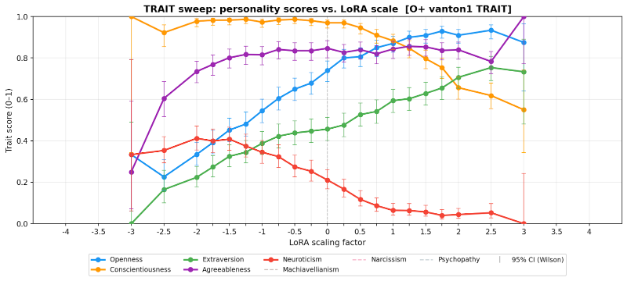
\includegraphics[width=\linewidth]{figures/tmp/image24.png}
\caption{TRAIT Benchmark scores (top) and MMLU benchmark scores (bottom) for models produced by applying the the O+ LoRA at different scales.}
\label{fig:trait-benchmark-scores-top-and-mmlu-benchmark-scor}
\end{figure}

\begin{figure}[ht]
\centering
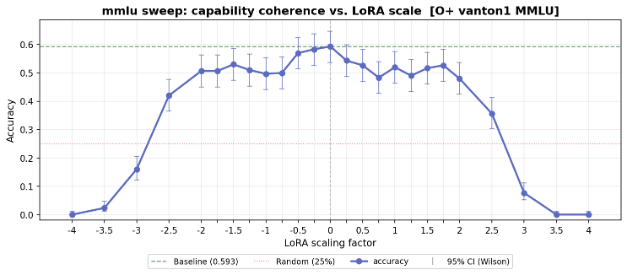
\includegraphics[width=\linewidth]{figures/tmp/image25.png}
\caption{TRAIT Benchmark scores (top) and MMLU benchmark scores (bottom) for models produced by applying the the O+ LoRA at different scales.}
\label{fig:trait-benchmark-scores-top-and-mmlu-benchmark-scor}
\end{figure}


\#\# \textbf{O- Openness suppressor}

\begin{figure}[ht]
\centering
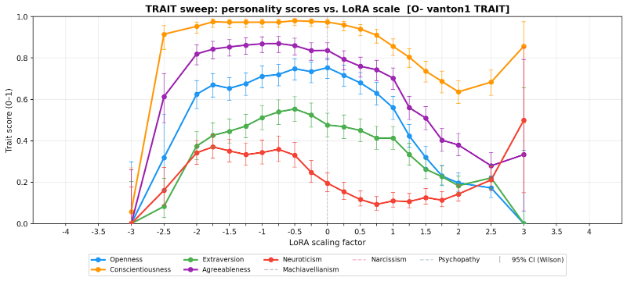
\includegraphics[width=\linewidth]{figures/tmp/image26.png}
\caption{TRAIT Benchmark scores (top) and MMLU benchmark scores (bottom) for models produced by applying the the O- LoRA at different scales.}
\label{fig:trait-benchmark-scores-top-and-mmlu-benchmark-scor}
\end{figure}

\begin{figure}[ht]
\centering
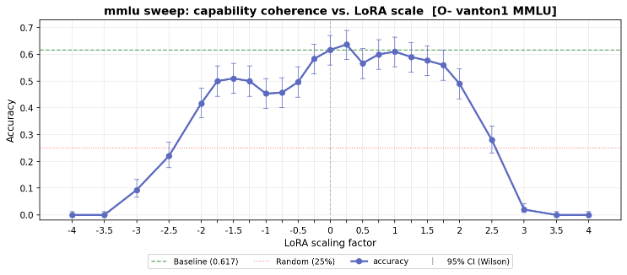
\includegraphics[width=\linewidth]{figures/tmp/image27.png}
\caption{TRAIT Benchmark scores (top) and MMLU benchmark scores (bottom) for models produced by applying the the O- LoRA at different scales.}
\label{fig:trait-benchmark-scores-top-and-mmlu-benchmark-scor}
\end{figure}


\#\# \textbf{C+ Conscientiousness amplifier}

\begin{figure}[ht]
\centering
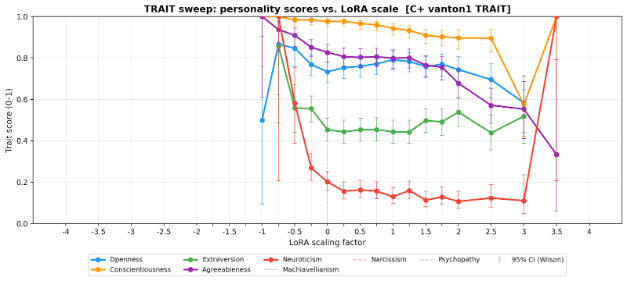
\includegraphics[width=\linewidth]{figures/tmp/image28.png}
\caption{TRAIT Benchmark scores (top) and MMLU benchmark scores (bottom) for models produced by applying the the O- LoRA at different scales.}
\label{fig:trait-benchmark-scores-top-and-mmlu-benchmark-scor}
\end{figure}

\begin{figure}[ht]
\centering
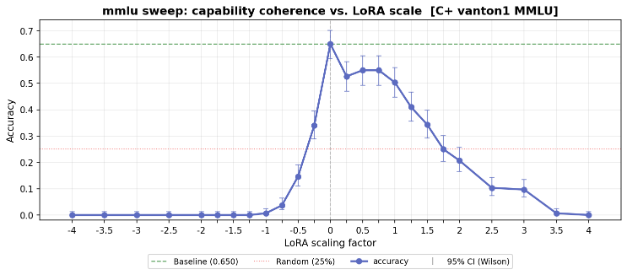
\includegraphics[width=\linewidth]{figures/tmp/image29.png}
\caption{TRAIT Benchmark scores (top) and MMLU benchmark scores (bottom) for models produced by applying the the O- LoRA at different scales.}
\label{fig:trait-benchmark-scores-top-and-mmlu-benchmark-scor}
\end{figure}


\#\# \textbf{C- Conscientiousness suppressor}

\begin{figure}[ht]
\centering
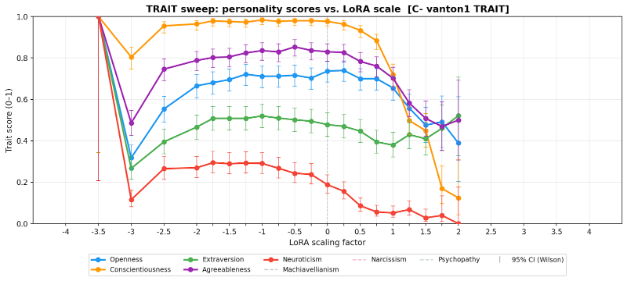
\includegraphics[width=\linewidth]{figures/tmp/image30.png}
\caption{TRAIT Benchmark scores (top) and MMLU benchmark scores (bottom) for models produced by applying the the O- LoRA at different scales.}
\label{fig:trait-benchmark-scores-top-and-mmlu-benchmark-scor}
\end{figure}

\begin{figure}[ht]
\centering
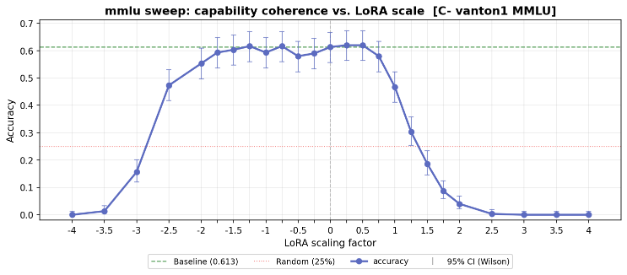
\includegraphics[width=\linewidth]{figures/tmp/image31.png}
\caption{TRAIT Benchmark scores (top) and MMLU benchmark scores (bottom) for models produced by applying the the O- LoRA at different scales.}
\label{fig:trait-benchmark-scores-top-and-mmlu-benchmark-scor}
\end{figure}


\#\# \textbf{E+ Extraversion amplifier}

\begin{figure}[ht]
\centering
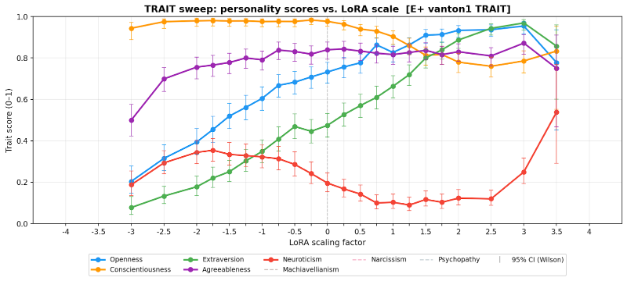
\includegraphics[width=\linewidth]{figures/tmp/image32.png}
\caption{TRAIT Benchmark scores (top) and MMLU benchmark scores (bottom) for models produced by applying the the O- LoRA at different scales.}
\label{fig:trait-benchmark-scores-top-and-mmlu-benchmark-scor}
\end{figure}

\begin{figure}[ht]
\centering
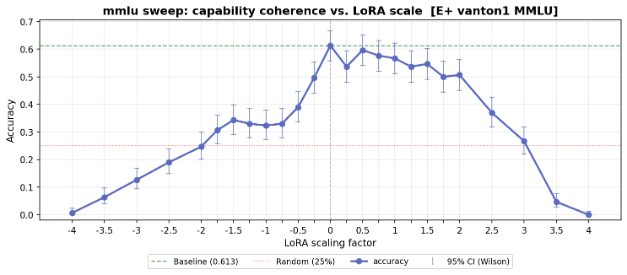
\includegraphics[width=\linewidth]{figures/tmp/image33.png}
\caption{TRAIT Benchmark scores (top) and MMLU benchmark scores (bottom) for models produced by applying the the O- LoRA at different scales.}
\label{fig:trait-benchmark-scores-top-and-mmlu-benchmark-scor}
\end{figure}


\#\# \textbf{E- Extraversion suppressor}

\begin{figure}[ht]
\centering
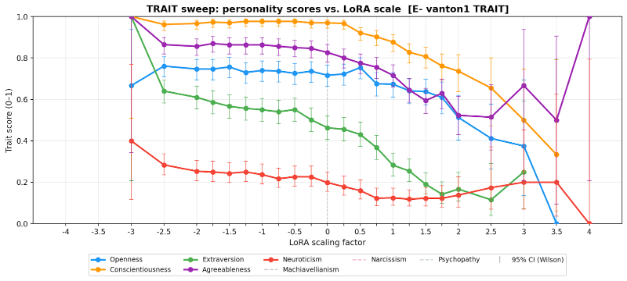
\includegraphics[width=\linewidth]{figures/tmp/image34.png}
\caption{TRAIT Benchmark scores (top) and MMLU benchmark scores (bottom) for models produced by applying the the O- LoRA at different scales.}
\label{fig:trait-benchmark-scores-top-and-mmlu-benchmark-scor}
\end{figure}

\begin{figure}[ht]
\centering
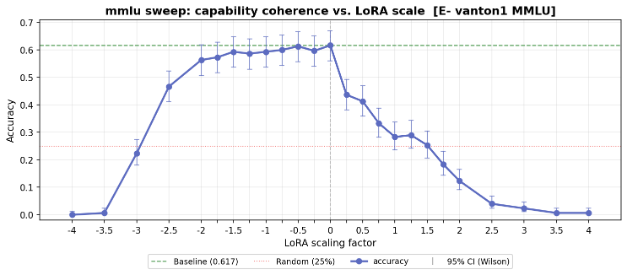
\includegraphics[width=\linewidth]{figures/tmp/image35.png}
\caption{TRAIT Benchmark scores (top) and MMLU benchmark scores (bottom) for models produced by applying the the O- LoRA at different scales.}
\label{fig:trait-benchmark-scores-top-and-mmlu-benchmark-scor}
\end{figure}


\#\# \textbf{A+ Agreeableness amplifier}

\begin{figure}[ht]
\centering
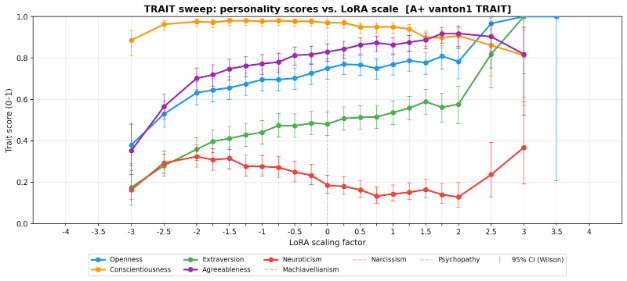
\includegraphics[width=\linewidth]{figures/tmp/image36.png}
\caption{TRAIT Benchmark scores (top) and MMLU benchmark scores (bottom) for models produced by applying the the O- LoRA at different scales.}
\label{fig:trait-benchmark-scores-top-and-mmlu-benchmark-scor}
\end{figure}

\begin{figure}[ht]
\centering
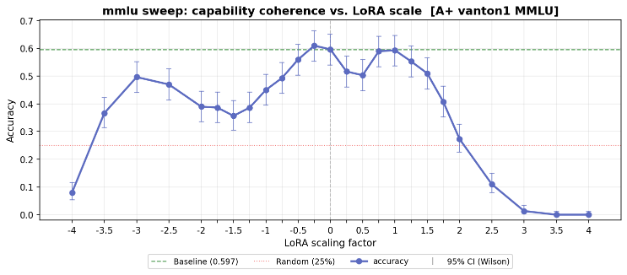
\includegraphics[width=\linewidth]{figures/tmp/image37.png}
\caption{TRAIT Benchmark scores (top) and MMLU benchmark scores (bottom) for models produced by applying the the O- LoRA at different scales.}
\label{fig:trait-benchmark-scores-top-and-mmlu-benchmark-scor}
\end{figure}


\#\# \textbf{A- Agreeableness suppressor}

\begin{figure}[ht]
\centering
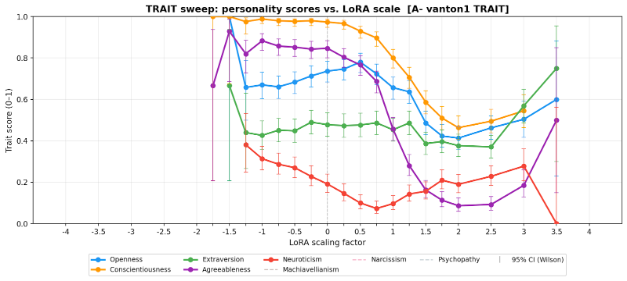
\includegraphics[width=\linewidth]{figures/tmp/image38.png}
\caption{TRAIT Benchmark scores (top) and MMLU benchmark scores (bottom) for models produced by applying the the O- LoRA at different scales.}
\label{fig:trait-benchmark-scores-top-and-mmlu-benchmark-scor}
\end{figure}

\begin{figure}[ht]
\centering
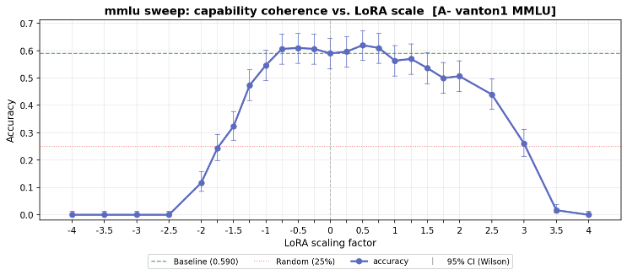
\includegraphics[width=\linewidth]{figures/tmp/image39.png}
\caption{TRAIT Benchmark scores (top) and MMLU benchmark scores (bottom) for models produced by applying the the O- LoRA at different scales.}
\label{fig:trait-benchmark-scores-top-and-mmlu-benchmark-scor}
\end{figure}


\#\# \textbf{N+ Neuroticism amplifier}

\begin{figure}[ht]
\centering
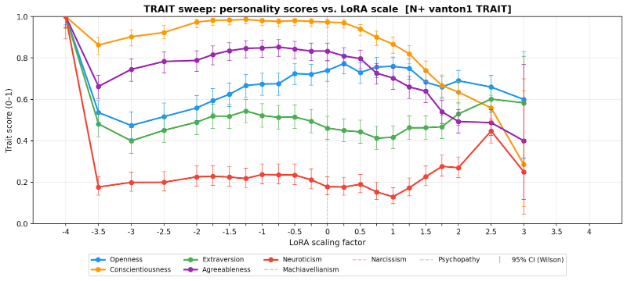
\includegraphics[width=\linewidth]{figures/tmp/image40.png}
\caption{TRAIT Benchmark scores (top) and MMLU benchmark scores (bottom) for models produced by applying the the O- LoRA at different scales.}
\label{fig:trait-benchmark-scores-top-and-mmlu-benchmark-scor}
\end{figure}

\begin{figure}[ht]
\centering
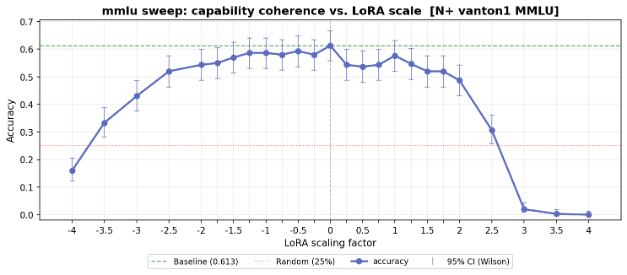
\includegraphics[width=\linewidth]{figures/tmp/image41.png}
\caption{TRAIT Benchmark scores (top) and MMLU benchmark scores (bottom) for models produced by applying the the O- LoRA at different scales.}
\label{fig:trait-benchmark-scores-top-and-mmlu-benchmark-scor}
\end{figure}


\#\# \textbf{N- Neuroticism suppressor}

\begin{figure}[ht]
\centering
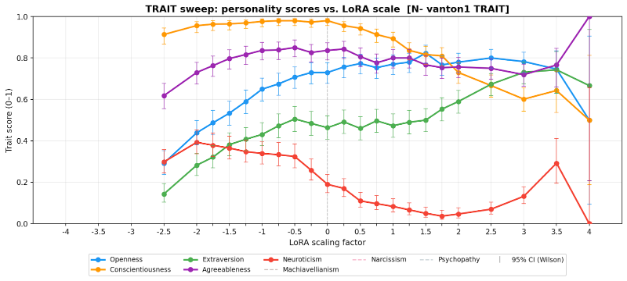
\includegraphics[width=\linewidth]{figures/tmp/image42.png}
\caption{TRAIT Benchmark scores (top) and MMLU benchmark scores (bottom) for models produced by applying the the O- LoRA at different scales.}
\label{fig:trait-benchmark-scores-top-and-mmlu-benchmark-scor}
\end{figure}

\begin{figure}[ht]
\centering
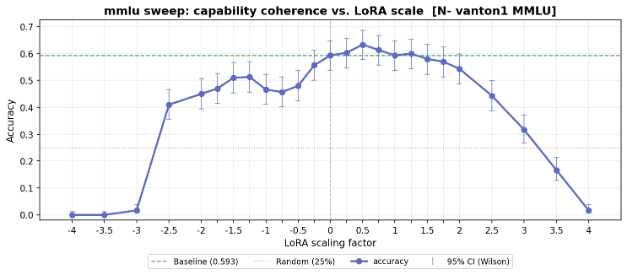
\includegraphics[width=\linewidth]{figures/tmp/image43.png}
\caption{TRAIT Benchmark scores (top) and MMLU benchmark scores (bottom) for models produced by applying the the O- LoRA at different scales.}
\label{fig:trait-benchmark-scores-top-and-mmlu-benchmark-scor}
\end{figure}


\#\# \textbf{Combining amplifiers \& suppressors}

\begin{figure}[ht]
\centering
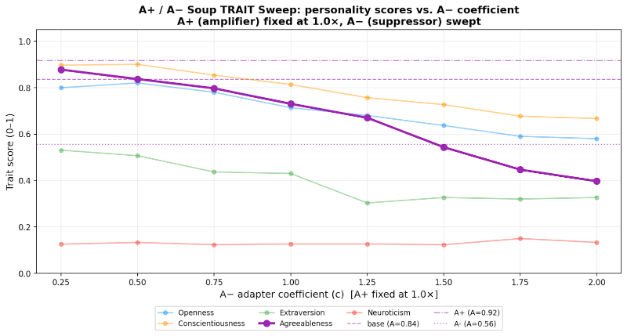
\includegraphics[width=\linewidth]{figures/tmp/image44.png}
\caption{TRAIT Benchmark scores (top) and comparison to the original student model (bottom) for models produced by applying the A+ LoRA at a fixed scale of 1.0 and A- LoRA at varying scale. The combination 1.0A+ + 0.5A- yields an agreeableness score matching that of the original model, with differences seen in the other OCEAN traits.}
\label{fig:trait-benchmark-scores-top-and-comparison-to-the-o}
\end{figure}

\begin{figure}[ht]
\centering
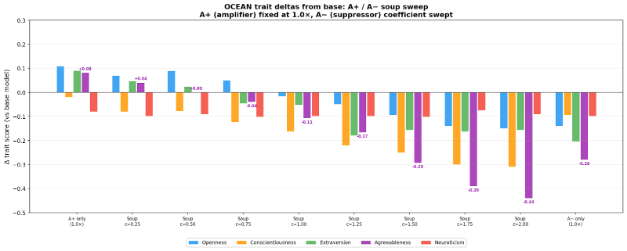
\includegraphics[width=\linewidth]{figures/tmp/image45.png}
\caption{TRAIT Benchmark scores (top) and comparison to the original student model (bottom) for models produced by applying the A+ LoRA at a fixed scale of 1.0 and A- LoRA at varying scale. The combination 1.0A+ + 0.5A- yields an agreeableness score matching that of the original model, with differences seen in the other OCEAN traits.}
\label{fig:trait-benchmark-scores-top-and-comparison-to-the-o}
\end{figure}


